\section*{Exercice 122 -- PFD}
\setcounter{exo}{0}
%CCS MP 2010

Le bras implanté sur le système ADVIA WorkCell R, est motorisé selon trois « axes » asservis (appelés « Axe 1 », « Axe 2 » et « Axe 3 » dans la suite) assurant les mouvements de type translation / rotation / translation.

\begin{center}
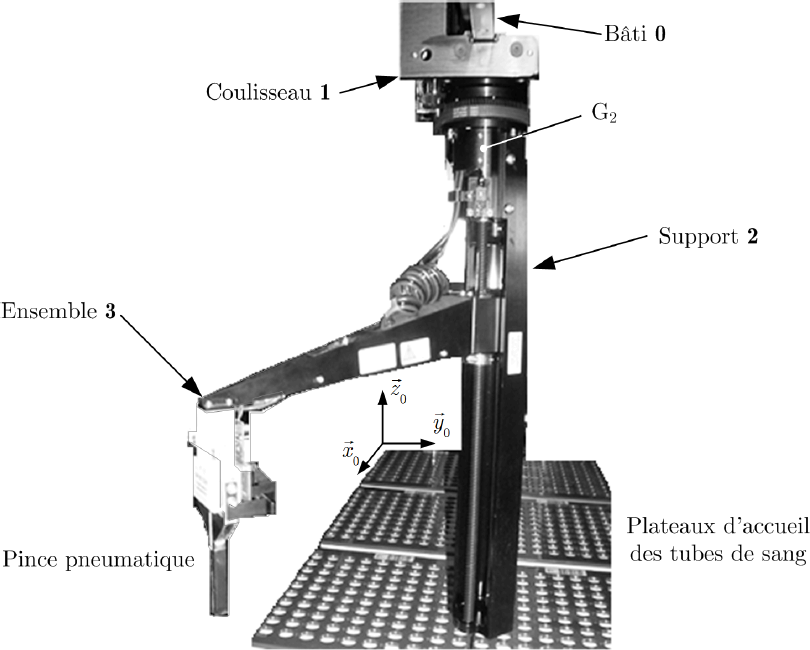
\includegraphics[width=\linewidth]{995_02}
\end{center}


Le bras est constitué de trois solides indéformables : Coulisseau 1, Support 2 et Ensemble bras + pince +
tube 3. Les mouvements autorisés entre ces solides sont associés aux trois axes du bras manipulateur et sont
paramétrés de la façon suivante.

\begin{center}
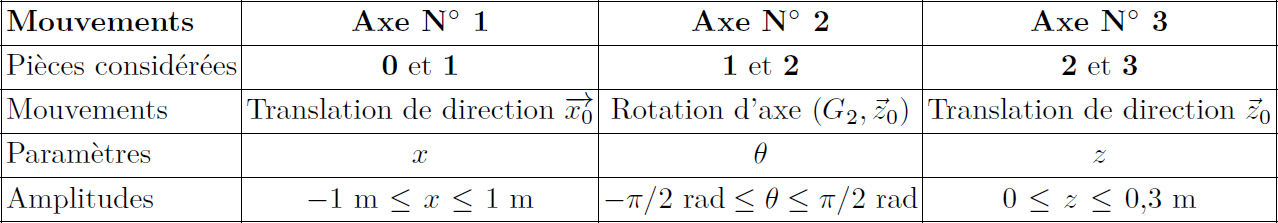
\includegraphics[width=\linewidth]{995_01}
\end{center}


Les amplitudes sont définies depuis la position de référence du bras, dans laquelle il se place après la prise
d’origine.
r
Les trois solides ont les caractéristiques suivantes.

\begin{center}
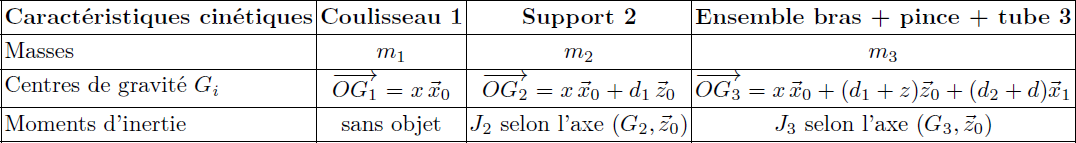
\includegraphics[width=\linewidth]{995_03}
\end{center}

L’orientation de la base $\base{x_1}{y_1}{z_1}$ par rapport à la base $\base{x_0}{y_0}{z_0}$ est définie par $\theta  = \angl{x_0}{x_1} = \angl{y_0}{y_1}$.
Valeurs numériques : $d_1 = \SI{0,2}{m}$, $d_2 + d = \SI{0,35}{m}$.
Pour chacun des trois axes motorisés, une action mécanique et un frottement visqueux équivalents de l’actionneur
$\left[ M_i \right]$ associé à l’axe $i$ sont définis au niveau de la liaison correspondante.


\begin{center}
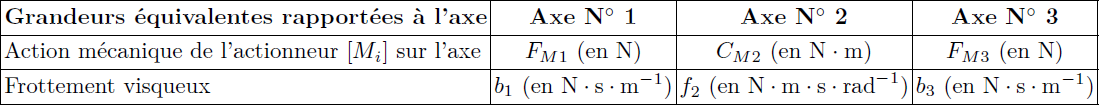
\includegraphics[width=\linewidth]{995_04}
\end{center}

Le « graphe des liaisons et des efforts » (encore appelé « graphe d’analyse ») du modèle mécanique du bras est
proposé figure suivante.


\begin{center}
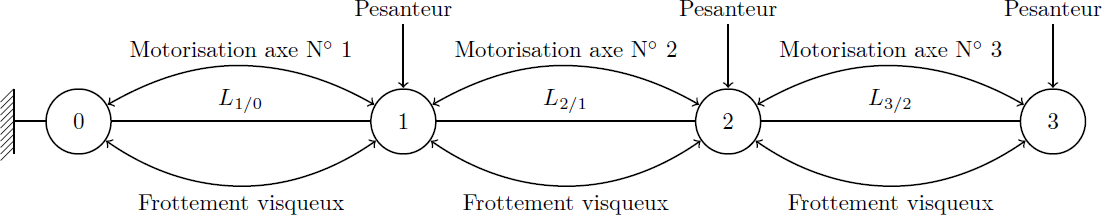
\includegraphics[width=\linewidth]{995_05}
\end{center}


\subparagraph{}
\textit{Proposer une stratégie d’isolements et de calculs à mettre en \oe{}uvre pour déterminer les expressions des
actions mécaniques $F_{M1}$, $C_{M2}$ et $F_{M3}$ (générées par les actionneurs $\left[ M_i \right]$ associés aux trois axes) : on indiquera, l’ensemble isolé, le théorème à utiliser (avec éventuellement le point de calcul) et la direction de projection en justifiant clairement le choix de la méthode adoptée.}
\ifprof
\begin{corrige}
\end{corrige}
\else
\fi

À partir de la stratégie d’isolements établie, on obtient les deux équations différentielles suivantes pour les
expressions des efforts $F_{M1}$ et $F_{M3}$ :
\begin{itemize}
\item équation (E1) : $F_{M1} = (m_1 + m_2 + m_3)\ddot{x} + b_1x\dot{x} - m_3\left( d_2 + d\right) \left(\ddot{\theta} \sin \theta +\dot{\theta}^2 \cos \theta \right)$;
\item équation (E3) : $F_{M3} = m_3\ddot{z}+b_3\dot{z}-m_3 g$.
\end{itemize}

\subparagraph{}
\textit{Montrer que l’équation différentielle (E2) reliant le couple $C_{M2}$, l’angle $\theta$, le déplacement $x$ et leurs dérivées
successives est de la forme $C_{M2}= A \ddot{\theta}+B\dot{\theta}+C\ddot{x}$ où les termes $A$, $B$ et $C$ seront exprimés en fonction des termes $m_3$, $J_2$, $J_3$, $d_2$, $d$, $f_2$ et $\theta$. Les différentes étapes du calcul seront précisément indiquées.}
\ifprof
\begin{corrige}
\end{corrige}
\else
\fi

Les évolutions dynamiques associées au bras motorisé lorsque les trois actionneurs sont commandés simultanément
sont donc décrites par les trois équations différentielles obtenues précédemment.




\subparagraph{}
\textit{À partir des équations précédentes, justifier que les mouvements de deux des axes sont couplés.
Le couplage des mouvements peut créer des accélérations transitoires importantes pouvant induire un risque de
débordement du sang du tube saisi par la pince en extrémité du bras à trois degrés de liberté.}
\ifprof
\begin{corrige}
\end{corrige}
\else
\fi
%
%
%
%
%\subparagraph{}
%\textit{}
%\ifprof
%\begin{corrige}
%\end{corrige}
%\else
%\fi
%
%
%
%\subparagraph{}
%\textit{}
%\ifprof
%\begin{corrige}
%\end{corrige}
%\else
%\fi
